\subsection{Secuenciación das actividades}
%• Desenvolvemento completo das diferentes sesións de clase, incluídos os anexos co material completo e necesario para aplicar a unidade didáctica.

Durante esta sección detallaremos as actividades que se desenvolverán durante esta unidade didáctica. Para o \citeA{dicionarioterminoscervantes}, as actividades son ``todas aquelas accións que realiza o alumno como parte do proceso instrutivo que segue, xa sexa na aula [...] ou en calquera outro lugar''. As actividades constituirán unidades de traballo dentro da nosa proposta didáctica.

En paralelo as actividades que imos describir a continuación, crearase un blogue onde se publicarán os contidos que se tratan na clase incorporando fontes de información adicionais como poden ser vídeos de YouTube onde se explican os mesmos contidos de forma diferente ou artigos doutras páxinas web. O obxectivo deste blogue é por unha parte que aqueles alumnos e alumnas que non puideron asistir á clase vexan o que se traballou durante ela e que por outra aqueles que desexen repasar poidan facelo vendo ademais o explicado dende outros puntos de vista. No Apéndice~\ref{fich:blogue} pódense ver as entradas que se publicaron neste blogue.

\subsubsection{Act. 0: Fotografando a xeometría}\label{act:fotografias}
Propoñeremos esta actividade como unha tarefa que o alumnado deberá realizar na casa. Trátase dunha actividade introdutoria na que deberán enviar por correo electrónico fotografías con elementos xeométricos que poidan atopar na súa contorna. Entregarémoslles unha ficha que se pode ver no  Apéndice~\ref{fich:act0} coas instrucións da actividade.

O obxectivo desta actividade é que os estudantes tomen conciencia de que está rodeados de obxectos matemáticos e ao mesmo tempo obter material co que poder traballar tanto para a posición relativa de rectas como para a clasificación de polígonos.

\begin{figure}[h!]
  \centering
  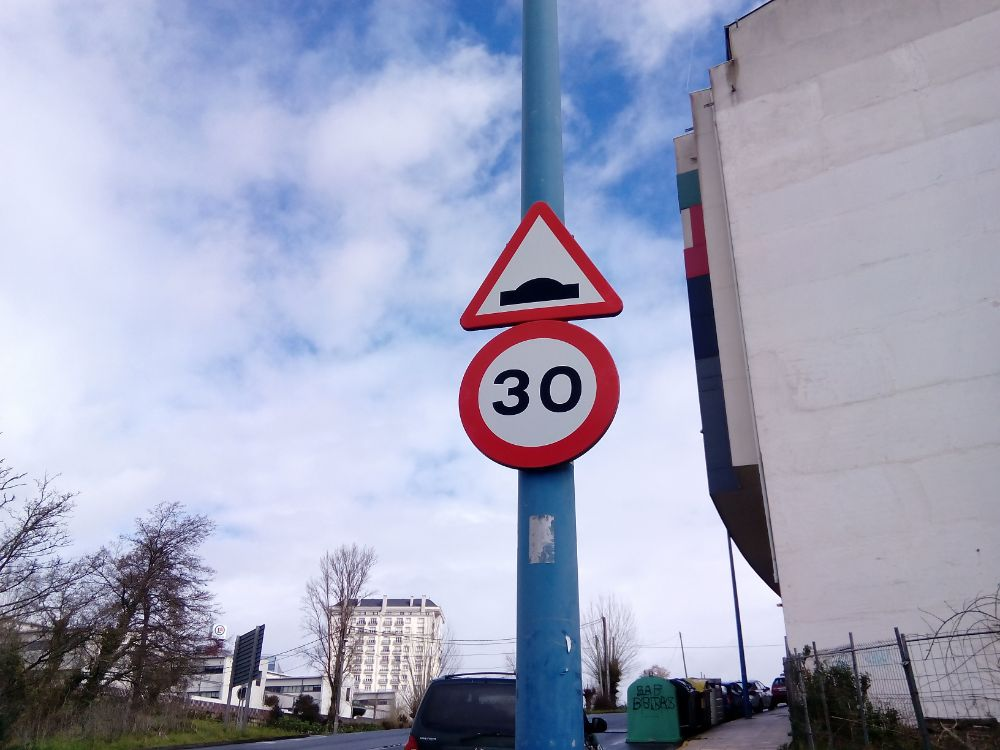
\includegraphics[height=4cm]{img/act0-1.jpg}
  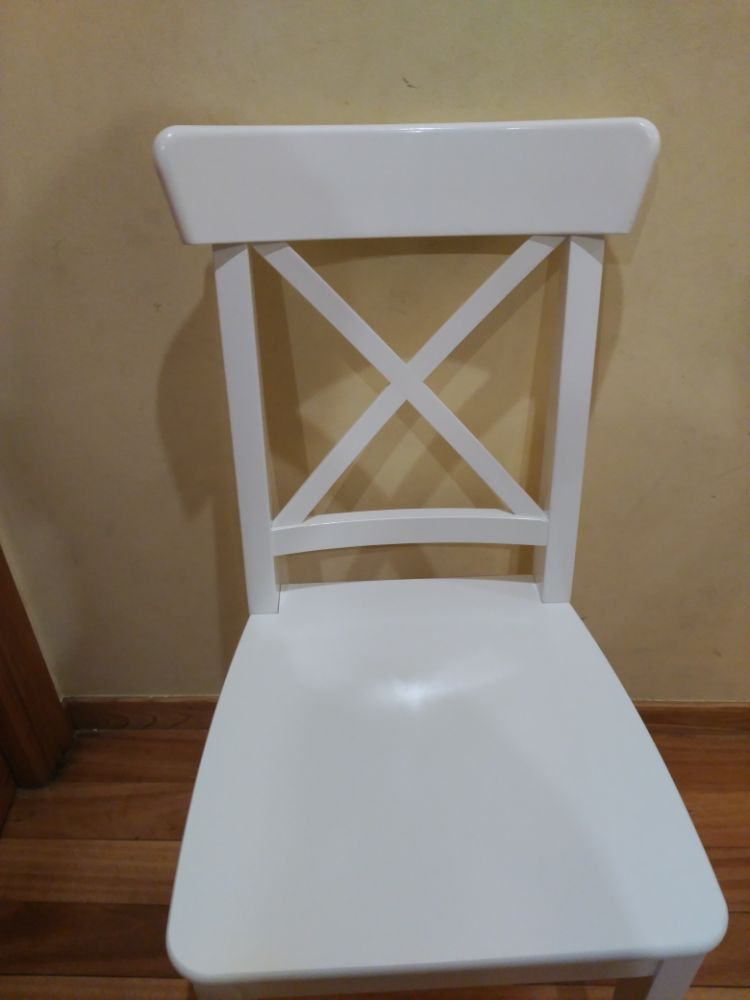
\includegraphics[height=4cm]{img/act0-2.jpg}
  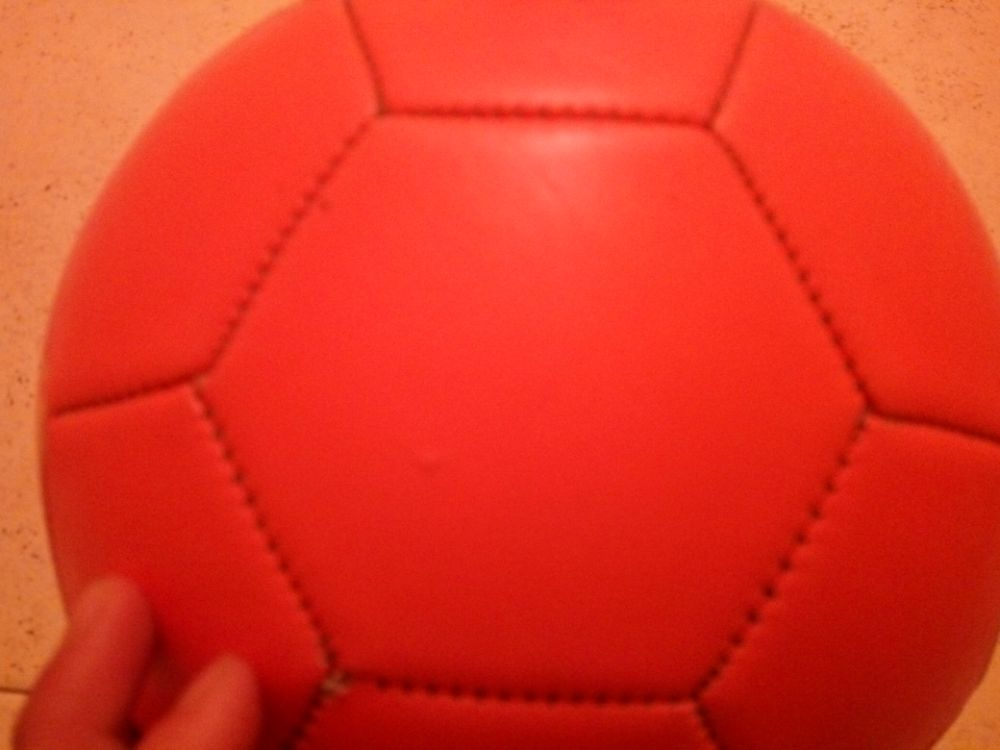
\includegraphics[height=4cm]{img/act0-3.jpg}
  \caption{Imaxes enviadas polos alumnos para a primeira actividade.}\label{fig:act0}
\end{figure}

Todas as fotos enviadas polo alumando serán subidas ao blogue da materia para poder traballas con elas en actividades posteriores. Na Figura~\ref{fig:act0} pódese ver algún exemplo do tipo de fotos que se buscan.

Dedicaremos entre 5 ou 10 minutos durante algún momento libre dunha unidade didáctica anterior a explicación desta actividade que os alumnos e alumnas deberán desenvolver na casa. O rol do profesor será nesta actividade de organizador pois o seu papel consistirá en explicar a actividade mentres que é o alumnado o que de forma autónoma deberá buscar que fotografiar e os medios para facelo.

\subsubsection{Act. 1: Xeometría}\label{act:xeometria}
Como primeira actividade realizaremos un pequeno coloquio onde os alumnos e alumnas intentarán dar definicións do que eles cren que se traballa na xeometría. A continuación, empregando os ordenadores portátiles buscarán definicións sobre este termo en internet e leranas en voz alta. O obxectivo que perseguimos con esta actividade é introducir ao alumnado nunha nova rama das matemáticas e, ao tempo, habitualos nunha nova dinámica de clase na que se buscan a interacción docente-discente.

Para a realización desta actividade de introdución-motivación empregaremos un total de 15 minutos. Neste caso, o docente terá un papel de promotor pois dirixirá un diálogo do alumnado sobre o que é a xeometría.

\subsubsection{Act.2: Puntos, liñas e posición relativa de liñas}\label{act:rectas}
Durante esta actividade empezaremos a explicar os elementos básicos de xeometría. En primeiro lugar, preguntarémoslle ao alumnado cal é para eles o elemento da xeometría máis simple que poden dicir. A raíz desta pregunta explicaremos o concepto de punto como elemento máis sinxelo e a partir del a recta, como unha sucesión de puntos aliñados, e o plano, como un conxunto de rectas e puntos aliñados. Empregando o programa GeoGebra verán que a recta é infinita e que polo tanto non ten principio nin fin. A continuación expoñeremos como se constrúe unha semirrecta, un segmento e detallaremos a clasificación de rectas en función da súa posición relativa.

Para practicar a posición relativa das rectas realizaremos un exercicio coas fotos de elementos xeométricos que enviaron na Actividade 0 (Sección~\ref{act:fotografias}). Dividiremos a clase en grupos e cada grupo deberá sinalar nas fotografías as rectas que sexan perpendiculares, secantes e paralelas. Para sinalar as rectas empregarase o programa de edición fotográfica, como pode ser GIMP.

\begin{figure}[h!]
  \centering
  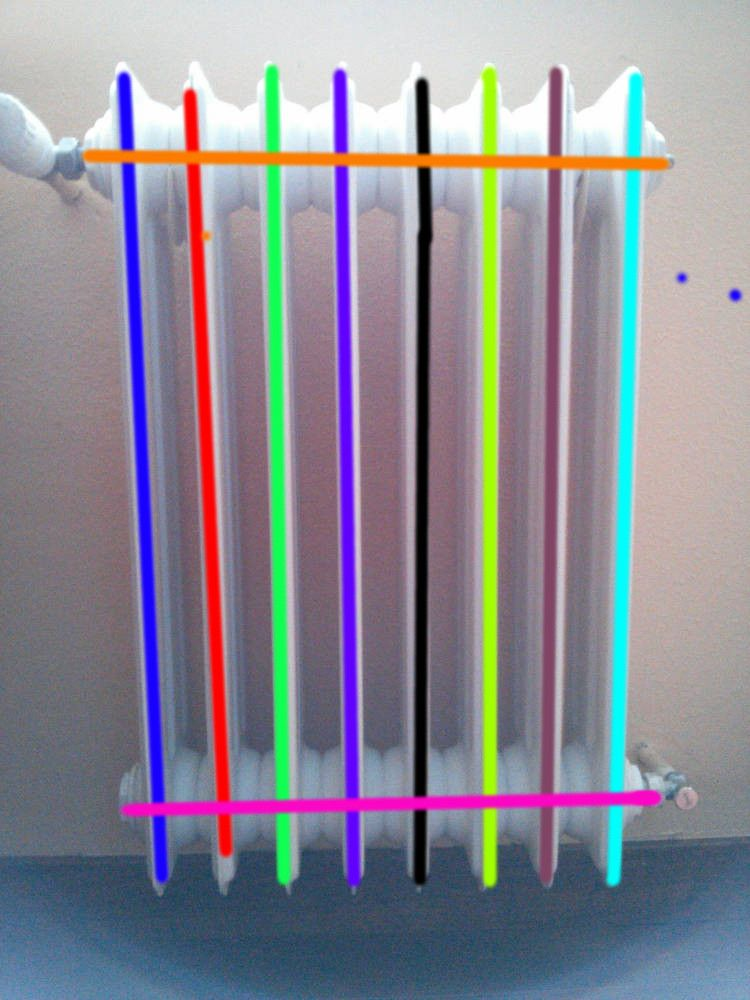
\includegraphics[height=4cm]{img/act1-img.jpg}
  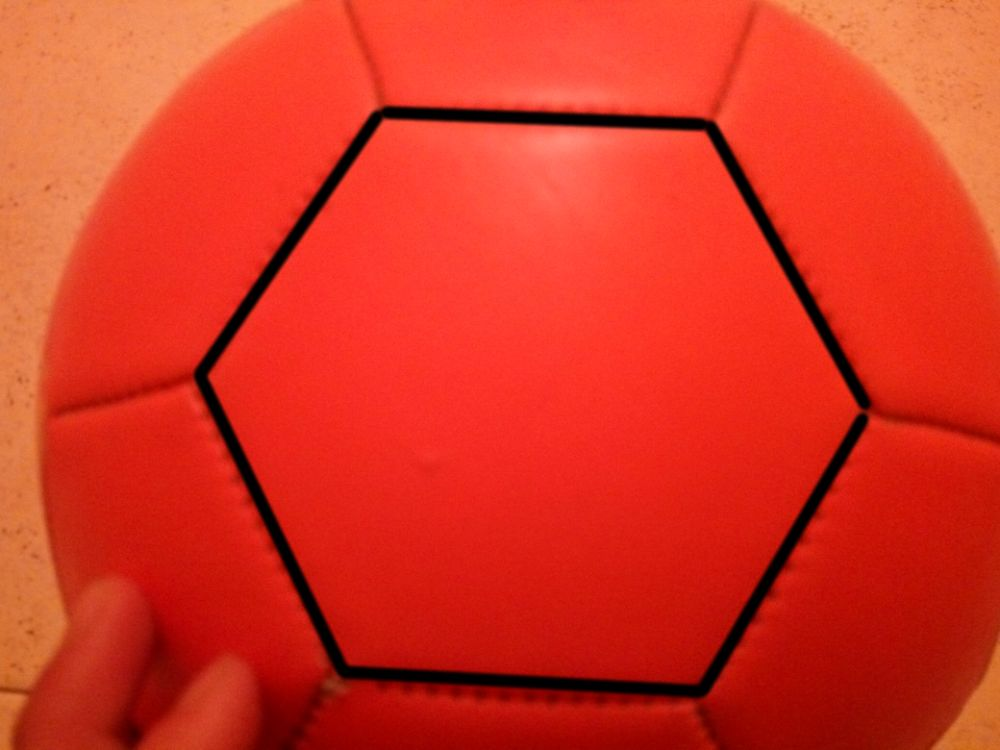
\includegraphics[height=4cm]{img/act1-img2.jpg}
  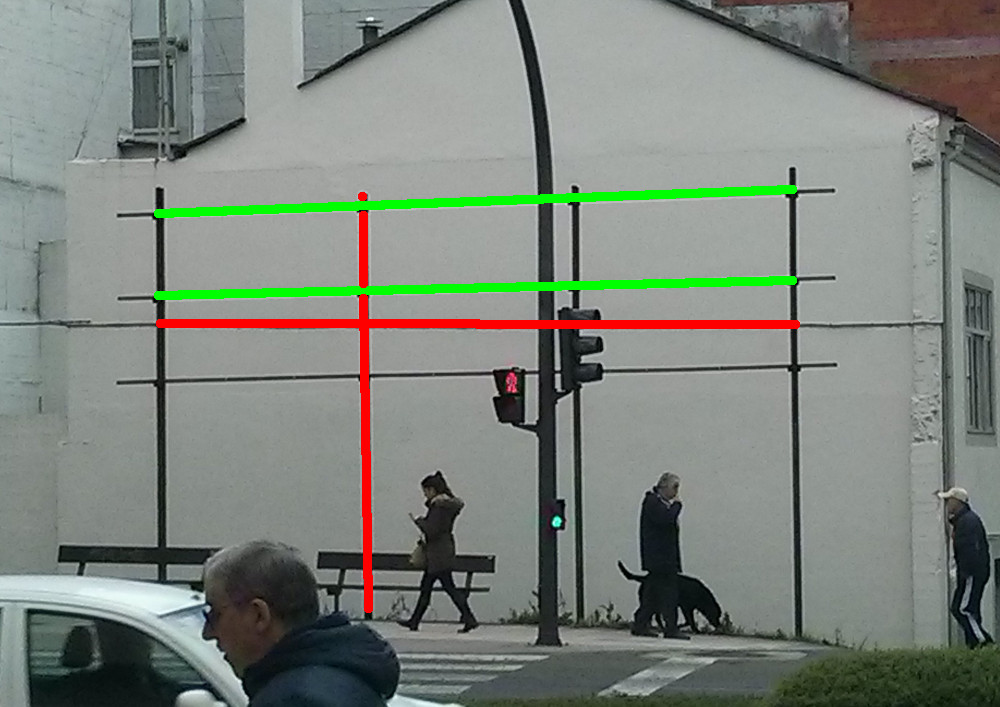
\includegraphics[height=4cm]{img/act1-img3.jpg}
  \caption{Marcado das imaxes con liñas paralelas, secantes e perpendiculares}\label{fig:act2}
\end{figure}

Despois de debuxar as rectas, os ficheiros serán gardados e enviados por correo electrónico ao profesor para ser proxectados na clase. Cada grupo deberá explicar porque as rectas seleccionadoras teñen unha clasificación ou outra. Na Figura~\ref{fig:act2} pódense ver exemplos do que se pretende acadar.

A duración desta actividade de desenvolvemento será de case dúas sesións (na primeira sesión tamén se realizará a Actividade 1). Nesta actividade o profesor adoptará varios papeis. Na primeira parte da actividade o papel será de controlador pois o profesor deberá explicar no encerado os novos conceptos por outro lado na actividade cos ordenadores o papel do profesor será de organizador pois explicará a actividade e deixará que os alumnos a realicen de forma autónoma mentres resolve as dúbidas que poidan xurdir.

\subsubsection{Act. 3: Ángulos, sistema sexasesimal e clasificación de ángulos en función da súa amplitude}\label{act:angulos}
Empezaremos esta actividade explicando o concepto de ángulo e as súas partes. Explicaremos que os ángulos se miden en función da súa amplitude e que para medilos empregamos o sistema sexasesimal. Explicamos o sistema sesaxesimal e como facer sumas e restas de grados expresados neste sistema. Baseamos a nosa explicación cunha comparación con algo que xa coñecen, a relación entre horas, minutos e segundos. Para practicar os cálculos co sistema sexasesimal, faremos varios exercicios e problemas propostos polo libro de texto. Despois de que se corrixan os exercicios, explicaremos a clasificación dos ángulos en función da súa amplitude. Para practicar esta clasificación faremos un pequeno xogo onde as e os estudantes deberán por grupos clasificar diversos ángulos xerados aleatoriamente polo web \href{http://random.org}{Random.org}.

%TODO: Engadir problemas sistema sexagesimal.

A duración desta actividade de desenvolvemento será de tres sesións. O papel do docente nesta actividade é de controlador, pois dirixirá a clase en todo momento deixando participar aos alumnos e alumnas só para a realización dos exercicios e o pequeno xogo do final da actividade.

\subsubsection{Act. 4: Mediatriz e bisectriz}\label{act:mediatriz}
Explicaremos os conceptos de mediatriz e de bisectriz e de como se trazan. Intentaremos incidir nas propiedades matemáticas que teñen a mediatriz e da bisectriz, é dicir, que os puntos destas dúas rectas equidistan dos extremos do segmento e dos lados do ángulo respectivamente. Estas propiedades serannos útiles máis tarde para explicar outros obxectos xeométricos como os puntos notables dos triángulos. Para practicar estes conceptos novos para o alumnado faremos os problemas que se poden ver no Apéndice~\ref{fich:mediatriz}, os exercicios faranse de forma individual ou en parellas e corrixirémolos antes de rematar a clase.

Empregaremos unha sesión en completar esta actividade de desenvolvemento. De igual forma que na actividade anterior o papel do profesor será de controlador pois dirixirá toda a actividade, intervindo o alumnado durante a corrección dos exercicios.

\subsubsection{Act. 5: Exame de xeometría básica}\label{act:examen1}
Faremos un exame do explicado ata o momento que abrangue os conceptos de punto, rectas, planos, posición relativa de rectas, ángulos, clasificación de ángulos e posición relativa deles, sistema sesaxesimal, mediatrices e bisectrices. O exame que puxemos pódese ver no Apéndice~\ref{fich:ex1a}.

Durante o día seguinte ao exame, corrixirémolo na clase, explicaremos os criterios de corrección e ensinarémoslles aos estudantes os exames corrixidos. Desta forma terán unha retroalimentación moi rápida do traballo que fixeron no exame.

A duración desta actividade de avaliación será de dúas sesións a propia do exame e a seguinte, onde o corrixiremos na clase. O profesor tomará un rol de avaliador durante esta actividade na que se medirá o grao de competencia do alumnado nos novos conceptos.

\subsubsection{Act. 6: Polígonos, triángulos e as súas clasificacións}\label{act:clastriangulos}
Expoñeremos os conceptos de liña poligonal, de polígono e as clasificacións de polígonos en función dos seus ángulos e do número de lados. A continuación explicaremos a clasificación dos triángulos en función dos seus ángulos e do número de lados iguais.

\begin{figure}[h!]
  \centering
  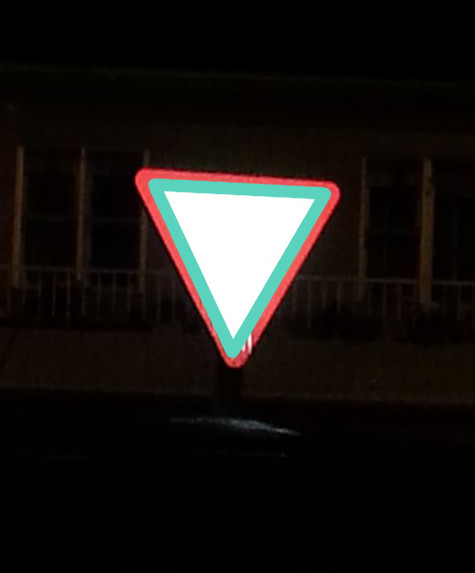
\includegraphics[height=4cm]{img/trian1.jpg}
  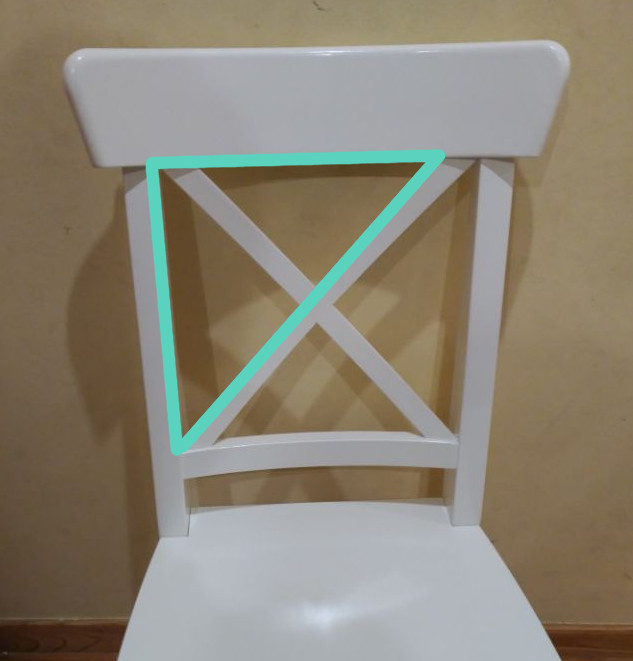
\includegraphics[height=4cm]{img/trian2.jpg}
  \caption{Exemplo de triángulo marcados sobre as fotografías}\label{fig:act7}
\end{figure}

Para practicar a clasificación dos triángulos realizaremos un exercicio coas fotos que entregaron os alumnos durante a Actividade 0 (Sección~\ref{act:fotografias}). Para isto dividiremos a clase en grupos de 2 ou 3 persoas e cada grupo cun ordenador deberá buscar 4 triángulos diferentes nas fotos enviadas polos compañeiros. Da mesma forma que na segunda actividade, o alumnado deberá enviar as fotos editadas cos triángulos marcados ao ordenador do profesor no que se proxectarán. Cada grupo saíra e explicará a clasificación de cada un dos triángulos que marcou. Na Figura~\ref{fig:act7} pódense ver algúns exemplos das figuras que se pretenden acadar neste exercicio.

A duración desta actividade de desenvolvemento será de case dúas sesións (dedicaremos a última parte da segunda sesión a Actividade 7). Os papeles que adopta o profesor durante esta actividade son o mesmo que na Actividade 2~(Sección~\ref{act:rectas}), na primeira parte controlará o proceso ensino-aprendizaxe mentras na segunda só a organizará deixando aos alumnos traballar de forma autónoma.

\subsubsection{Act. 7: Suma dos ángulos dun triángulo}\label{act:sumangulos}
Nesta pequena actividade explicaremos e demostraremos de forma gráfica que a suma dos ángulos dun triángulo da sempre 180 graos. Para iso unha vez explicada esta propiedade no encerado, repartiremos triángulos feitos con goma-eva, pero que están partidos en tres fragmento de forma que se pode ver como poñendo os ángulos de forma consecutiva, obtense un ángulo llano.

A duración desta actividade de desenvolvemento será de 10 minutos. Durante esta actividade, o papel do profesor será de controlador, pois será el quen dirixa todo o proceso.

\subsubsection{Act. 8: Puntos e rectas notables do triángulo}\label{act:rectasnotables}
Explicaremos os puntos e rectas notables dos triángulos. Empezaremos recordando as definicións matemáticas explicadas de mediatriz (como recta cuxos puntos equidistan dos extremos do segmento) e de bisectriz (como recta cuxos puntos equidistan dos lados do ángulo). Unha vez se repasaron estes conceptos, para explicar o circuncentro formulamos un problema no cal deberán buscar a posición ideal para colocar unha antena WiFi que abasteza ao instituto e a un hospital e centro comercial próximos. A formulación do problema acompoñámola coa primeira imaxe que se pode ver no Apéndice~\ref{fich:notables}.

Pediremos que os alumnos e as alumnas expoñan como calcularían ese punto e as razóns por que pensan que a súa solución é a adecuada. Trazaremos as solucións propostas no ordenador empregando o programa GeoGebra. Iremos explicando porque as solucións propostas son ou non correctas e no caso de que non xurda a resposta explicaremos porque a solución correcta consiste en trazar as mediatrices.

Para a explicación do dos demais puntos e rectas notables, empregaremos métodos similares como poden ser pedirlles que calculen onde situar unha corda para trazar a circunferencia interior dun triángulo coa segunda imaxe que se pode ver no Apéndice~\ref{fich:notables} explicando desta forma o incentro ou pedindo que dividan o triángulo en 6 partes de igual área no caso do baricentro.

A duración desta actividade de desenvolvemento será de dúas sesión. O papel do profesor durante esta actividade será unha mestura entre controlador e organizador pois mentres el dirixe a actividade, intentará organizar un diálogo entre o alumnado e entre o alumnado e o profesor, de forma que sexan eles e elas quen descubran como calcular os puntos dos problemas propostos.

\subsubsection{Act. 9: Teorema de Pitágoras}\label{act:pitagoras}
Explicaremos a denominación dos lados dun triángulo rectángulo e a relación entre a lonxitude destes. Para que os estudantes o vexan de forma gráfica, relacionaremos a relación entre os seus lados coa relación entre as áreas de cadrados con lados a hipotenusa e cada un dos catetos explicando que, segundo o teorema, cúmprese que a área do cadrado  que ten como lado a hipotenusa é igual a suma das áreas dos cadrados que teñen como lados os dous catetos.

Para reforzar o que explicamos no encerado proxectaremos varios fragmentos do documental \emph{Pitágoras: Mucha más que un teorema}\footnote{Este documental forma parte da serie Universo Matemático feito por RTVE que se pode ver completa en \href{http://www.rtve.es/television/la-aventura-del-saber/documentales/universo-matematico/}{rtve.es/television/la-aventura-del-saber/documentales/universo-matematico}.} relativos ao teorema. Ademais tamén se proxectará unha demostración feita con auga do teorema encontrada nun vídeo en YouTube\footnote{Pódese ver en \href{https://www.youtube.com/watch?v=1er3cHAWwIM}{youtube.com/watch?v=1er3cHAWwIM}.}. Despois de ver estas demostracións, faremos problemas da ficha que se pode ver no Apéndice~\ref{fich:pitagoras} e outros propostos polo libro de texto.

%TODO:Mirar outros exercicios.

A duración desta actividade de desenvolvemento será de dúas sesións dedicando a segunda á corrección dos problemas propostos. Durante esta actividade ao igual que pasaba nas Actividades~3~(Sección~\ref{act:angulos}) e 4~(Sección~\ref{act:mediatriz}), o papel do profesor será o de controlador deixando intervir ao alumando na resolución dos exercicios propostos.

\subsubsection{Act. 10: Clasificación cuadriláteros}\label{act:cuadrilateros}
Explicaremos a clasificación dos cuadriláteros en función das súas propiedades e para reforzar a nomenclatura, repetiremos o mesmo exercicio que se realizou para practicar a clasificación dos triángulos mais desta volta para practicar os cuadriláteros. Na Figura~\ref{fig:act11} pódese ver algún exemplo das imaxes que pretendemos acadar neste caso.

\begin{figure}[h!]
  \centering
  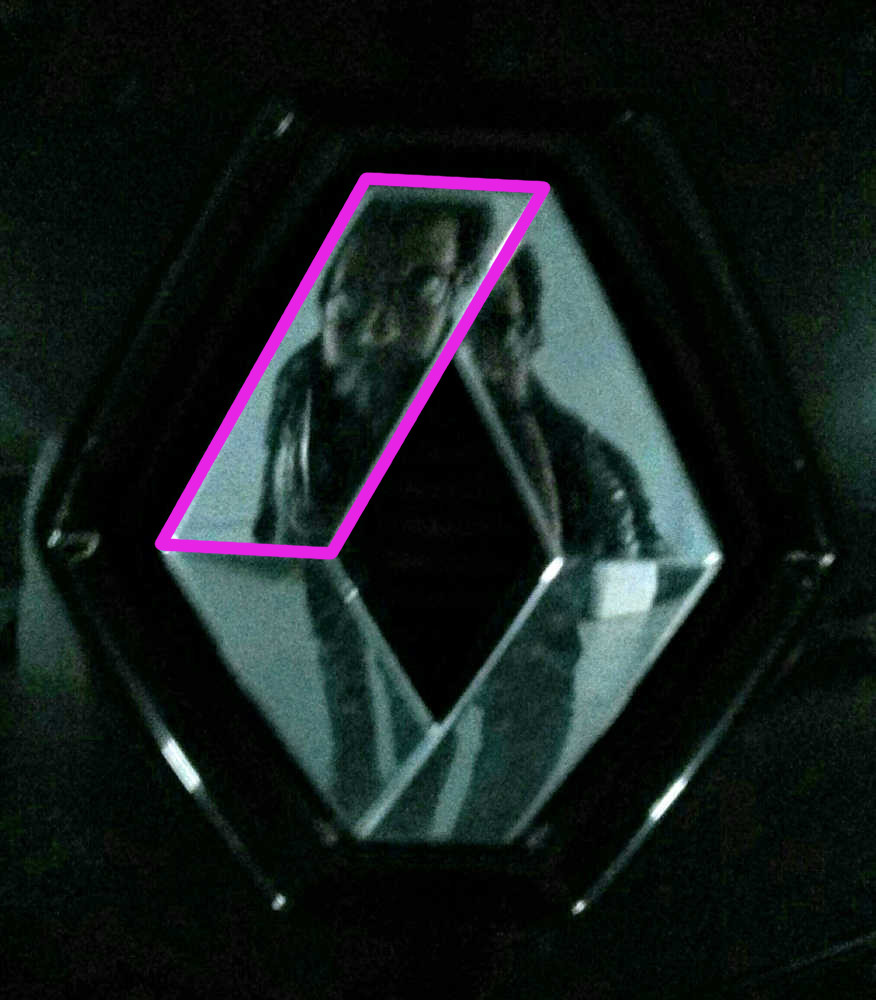
\includegraphics[height=4cm]{img/cuad1.jpg}
  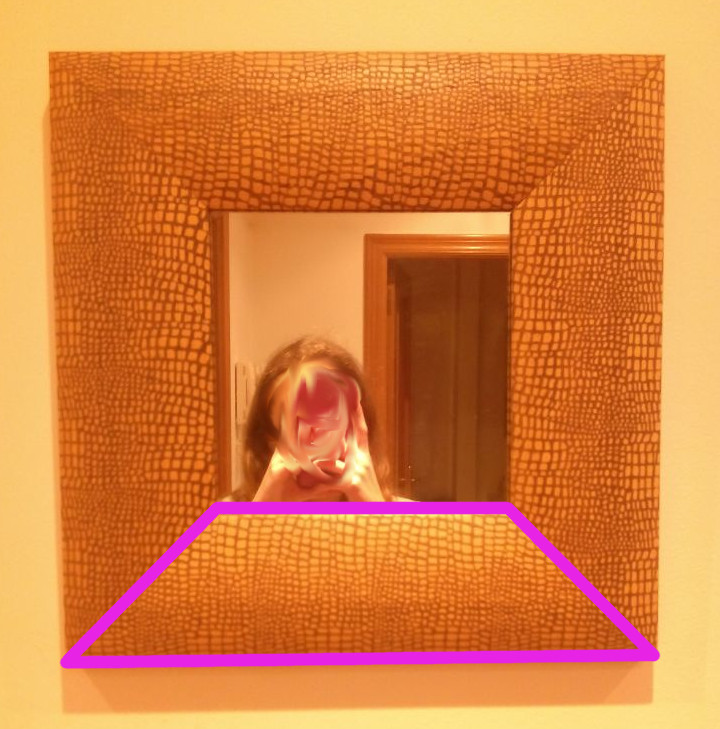
\includegraphics[height=4cm]{img/cuad2.jpg}
  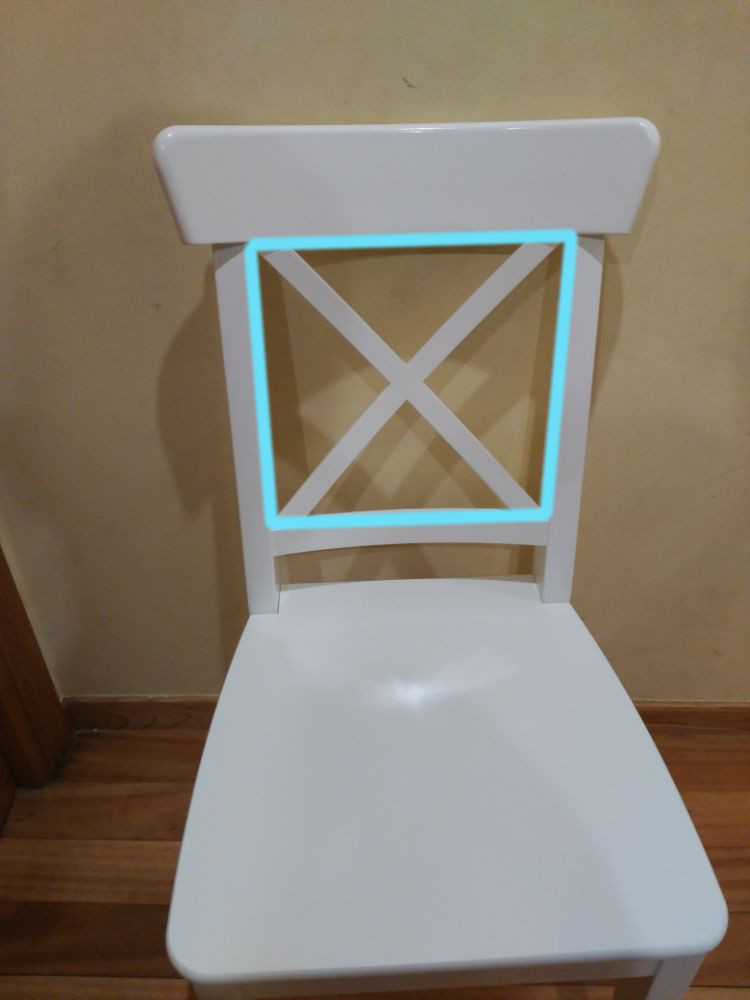
\includegraphics[height=4cm]{img/cuad3.jpg}
  \caption{Exemplo de cuadriláteros marcados sobre as fotografías}\label{fig:act11}
\end{figure}

A duración desta actividade de desenvolvemento será de dúas sesións. Esta actividade, ao ser copia da Actividade~6~(Sección~\ref{act:clastriangulos}), o profesor terá os mesmos papeis, controlador durante a exposición e organizador durante o exercicio.

\subsubsection{Act. 11: Elementos dos polígonos regulares. Circunferencia e círculo}\label{act:elementos}
%TODO: intentar mellorar actividade
Durante esta actividade explicaremos algún dos elementos dos polígonos regulares como o radio ou a apotema. Para explicar o concepto de circunferencia pedirémoslles ás alumnas e alumnos que formulen as súas propias definicións para ir corrixíndoas e terminar dando cunha correcta. Explicaremos os elementos da circunferencia e por último o círculo e os seus elementos.

A duración desta actividade de desenvolvemento será dunha sesión. O rol do profesor durante esta actividade será a de controlador pois será el quen dirixa todo o proceso ensino-aprendizaxe.

\subsubsection{Act. 12: Trívial de polígonos}\label{act:trivial}
Para practicar todos os conceptos traballados nas leccións anteriores realizaremos un trívial de 70 preguntas onde se repasará todo o aprendido. Para facer isto empregamos a plataforma Socrative\footnote{Pódese acceder a ela en \href{http://www.socrative.com/}{socrative.com}.} que dispón dunha aplicativo móbil para a realización dos test, así como a súa páxina web onde se pode seguir o proceso do alumnado. Como se pode ver no Apéndice~\ref{fich:trivial}, as preguntas formuladas eran de varios tipos: encontramos preguntas onde o alumnado debía seleccionar unha opción entre varias alternativas que lle eran dadas, preguntas onde debían dicir se un enunciado era correcto ou falso e preguntas onde eles mesmos debían escribir a resposta.

Para a realización do test dividiremos a clase en parellas e cada parella empregará un ordenador. Conectaranse á plataforma de Socrative e responderán a todas as preguntas durante a duración da clase. Durante a sesión seguinte a realización do trivial, analizaremos pregunta a pregunta cal é o resultado correcto e o porqué. Centrarémonos máis nos contidos que fallou a maior parte da clase.

A duración total desta actividade de consolidación será de dúas sesións. Nesta actividade o profesor actuará como organizador explicando a actividade e deixando ao alumnado traballar de forma autónoma.

\subsubsection{Act. 13: Exame polígonos}\label{act:examen2}
Realizaremos un exame dos contidos traballados dende o anterior exame. O exame pode verse no Apéndice~\ref{fich:ex2}. Da mesma forma que fixemos no primeiro exame, corrixiremos os exames durante esa tarde para amosarllos ao día seguinte corrixidos e que reciban o \emph{feedback} o máis cedo posible.

Desta forma esta actividade de avaliación terá unha duración de dúas sesións. Durante o segundo exame o profesor actuará de avaliador de forma que non intervirá ata que a tarefa proposta se complete.
